\documentclass[multi=tikzpicture,border=8pt]{standalone}
\usepackage[UTF8]{ctex}
\usepackage{amsmath,amssymb,tikz}
\usetikzlibrary{arrows.meta,calc}
\definecolor{blue}{HTML}{17365D}
\definecolor{red}{HTML}{AC3931}
\tikzset{every node/.style={font=\small},arrow/.style={-{Stealth[length=2.8mm]},thick},dim/.style={|<->|,thin},box/.style={draw,rounded corners,align=center,minimum width=2.5cm,minimum height=.8cm}}
\begin{document}
\begin{tikzpicture}

\draw[arrow](-3,0)--(4.2,0)node[right]{母粒子原方向};\fill[blue](0,0)circle(4pt)node[below]{$\pi^0$};\draw[arrow,blue](-3,0)--(-.5,0)node[above,midway]{$0.2c$};\draw[arrow,red](0,0)--(3,1.732)node[right]{$e^-$};\draw[arrow](0,0)--(-1,2.3)node[above]{$e^+$};\draw[arrow](0,0)--(1,-2)node[below]{$\gamma$};\draw(.9,0)arc(0:30:.9);\node[right]at(1,.35){$30^\circ$};\node[below]at(0,-3){未观测的两条方向仅为示意};

\end{tikzpicture}
\begin{tikzpicture}

\node[box](a)at(0,0){母粒子四动量$P$};\node[box,fill=red!8](b)at(5,0){已测电子$p_e$};\node[box,fill=blue!8](c)at(2.5,-2){剩余系统$Q=P-p_e$\\$Q^2>m^2$};\draw[arrow](a)--(c);\draw[arrow](b)--(c);\node[below]at(2.5,-3.2){非零光子使不变质量严格大于$m$};

\end{tikzpicture}
\begin{tikzpicture}
\draw[arrow](0,0)--(6.8,0)node[right]{$E/(\mathrm{MeV})$};\draw[arrow](0,0)--(0,5.3)node[above]{$E-b\sqrt{E^2-m^2}$};\draw[very thick,blue] plot coordinates {(0.03931,0.03407) (0.07119,0.05279) (0.10308,0.07503) (0.13497,0.09759) (0.16685,0.12026) (0.19874,0.14300) (0.23062,0.16576) (0.26251,0.18855) (0.29440,0.21135) (0.32628,0.23416) (0.35817,0.25697) (0.39005,0.27979) (0.42194,0.30262) (0.45383,0.32545) (0.48571,0.34828) (0.51760,0.37111) (0.54948,0.39395) (0.58137,0.41678) (0.61326,0.43962) (0.64514,0.46246) (0.67703,0.48530) (0.70891,0.50814) (0.74080,0.53098) (0.77268,0.55382) (0.80457,0.57666) (0.83646,0.59951) (0.86834,0.62235) (0.90023,0.64519) (0.93211,0.66804) (0.96400,0.69088) (0.99589,0.71372) (1.02777,0.73657) (1.05966,0.75941) (1.09154,0.78226) (1.12343,0.80510) (1.15532,0.82795) (1.18720,0.85079) (1.21909,0.87364) (1.25097,0.89649) (1.28286,0.91933) (1.31475,0.94218) (1.34663,0.96502) (1.37852,0.98787) (1.41040,1.01072) (1.44229,1.03356) (1.47418,1.05641) (1.50606,1.07925) (1.53795,1.10210) (1.56983,1.12495) (1.60172,1.14779) (1.63361,1.17064) (1.66549,1.19349) (1.69738,1.21633) (1.72926,1.23918) (1.76115,1.26203) (1.79304,1.28487) (1.82492,1.30772) (1.85681,1.33057) (1.88869,1.35342) (1.92058,1.37626) (1.95247,1.39911) (1.98435,1.42196) (2.01624,1.44480) (2.04812,1.46765) (2.08001,1.49050) (2.11190,1.51335) (2.14378,1.53619) (2.17567,1.55904) (2.20755,1.58189) (2.23944,1.60473) (2.27133,1.62758) (2.30321,1.65043) (2.33510,1.67328) (2.36698,1.69612) (2.39887,1.71897) (2.43076,1.74182) (2.46264,1.76467) (2.49453,1.78751) (2.52641,1.81036) (2.55830,1.83321) (2.59019,1.85606) (2.62207,1.87890) (2.65396,1.90175) (2.68584,1.92460) (2.71773,1.94745) (2.74961,1.97029) (2.78150,1.99314) (2.81339,2.01599) (2.84527,2.03884) (2.87716,2.06168) (2.90904,2.08453) (2.94093,2.10738) (2.97282,2.13023) (3.00470,2.15308) (3.03659,2.17592) (3.06847,2.19877) (3.10036,2.22162) (3.13225,2.24447) (3.16413,2.26731) (3.19602,2.29016) (3.22790,2.31301) (3.25979,2.33586) (3.29168,2.35870) (3.32356,2.38155) (3.35545,2.40440) (3.38733,2.42725) (3.41922,2.45010) (3.45111,2.47294) (3.48299,2.49579) (3.51488,2.51864) (3.54676,2.54149) (3.57865,2.56433) (3.61054,2.58718) (3.64242,2.61003) (3.67431,2.63288) (3.70619,2.65573) (3.73808,2.67857) (3.76997,2.70142) (3.80185,2.72427) (3.83374,2.74712) (3.86562,2.76996) (3.89751,2.79281) (3.92940,2.81566) (3.96128,2.83851) (3.99317,2.86136) (4.02505,2.88420) (4.05694,2.90705) (4.08883,2.92990) (4.12071,2.95275) (4.15260,2.97559) (4.18448,2.99844) (4.21637,3.02129) (4.24826,3.04414) (4.28014,3.06699) (4.31203,3.08983) (4.34391,3.11268) (4.37580,3.13553) (4.40769,3.15838) (4.43957,3.18123) (4.47146,3.20407) (4.50334,3.22692) (4.53523,3.24977) (4.56712,3.27262) (4.59900,3.29547) (4.63089,3.31831) (4.66277,3.34116) (4.69466,3.36401) (4.72655,3.38686) (4.75843,3.40970) (4.79032,3.43255) (4.82220,3.45540) (4.85409,3.47825) (4.88597,3.50110) (4.91786,3.52394) (4.94975,3.54679) (4.98163,3.56964) (5.01352,3.59249) (5.04540,3.61534) (5.07729,3.63818) (5.10918,3.66103) (5.14106,3.68388) (5.17295,3.70673) (5.20483,3.72958) (5.23672,3.75242) (5.26861,3.77527) (5.30049,3.79812) (5.33238,3.82097) (5.36426,3.84382) (5.39615,3.86666) (5.42804,3.88951) (5.45992,3.91236) (5.49181,3.93521) (5.52369,3.95806) (5.55558,3.98090) (5.58747,4.00375) (5.61935,4.02660) (5.65124,4.04945) (5.68312,4.07229) (5.71501,4.09514) (5.74690,4.11799) (5.77878,4.14084) (5.81067,4.16369) (5.84255,4.18653) (5.87444,4.20938) (5.90633,4.23223) (5.93821,4.25508) (5.97010,4.27793) (6.00198,4.30077) (6.03387,4.32362) (6.06576,4.34647) (6.09764,4.36932) (6.12953,4.39217) (6.16141,4.41501) (6.19330,4.43786) (6.22519,4.46071) (6.25707,4.48356) (6.28896,4.50641) (6.32084,4.52925) (6.35273,4.55210) (6.38462,4.57495)};\draw[red,dashed](0,4.40908)--(6.3,4.40908);\fill[red](6.15313,4.40908)circle(3pt);\draw[dashed](6.15313,0)--(6.15313,4.40908);\node[below]at(6.15313,0){79.99074};\node[left]at(0,4.40908){66.13622};\node[blue]at(3,3.4){曲线低于红线为允许区间};
\end{tikzpicture}
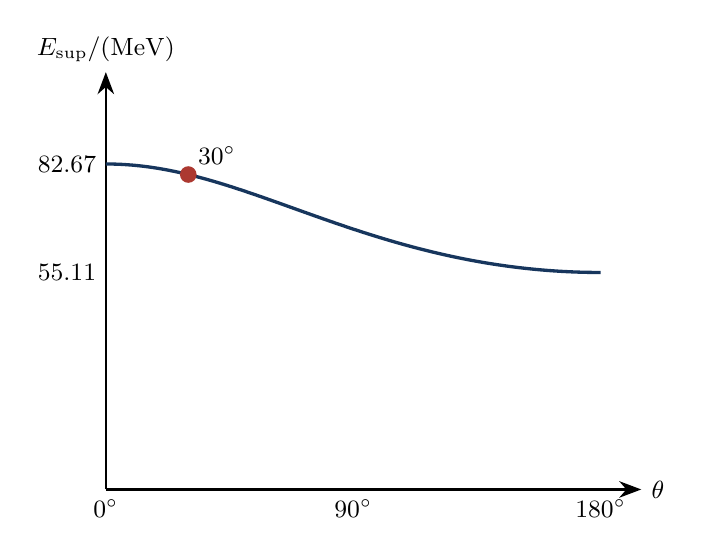
\begin{tikzpicture}
\draw[arrow](0,0)--(6.8,0)node[right]{$\theta$};\draw[arrow](0,0)--(0,5.3)node[above]{$E_{\rm sup}/(\mathrm{MeV})$};\draw[very thick,blue] plot coordinates {(0.00000,4.13349) (0.03510,4.13334) (0.07020,4.13286) (0.10530,4.13206) (0.14041,4.13095) (0.17551,4.12952) (0.21061,4.12778) (0.24571,4.12572) (0.28081,4.12335) (0.31591,4.12067) (0.35102,4.11768) (0.38612,4.11439) (0.42122,4.11079) (0.45632,4.10689) (0.49142,4.10269) (0.52652,4.09820) (0.56163,4.09341) (0.59673,4.08834) (0.63183,4.08298) (0.66693,4.07734) (0.70203,4.07143) (0.73713,4.06524) (0.77224,4.05879) (0.80734,4.05208) (0.84244,4.04510) (0.87754,4.03787) (0.91264,4.03040) (0.94774,4.02268) (0.98284,4.01472) (1.01795,4.00653) (1.05305,3.99812) (1.08815,3.98948) (1.12325,3.98063) (1.15835,3.97157) (1.19345,3.96230) (1.22856,3.95284) (1.26366,3.94319) (1.29876,3.93335) (1.33386,3.92333) (1.36896,3.91314) (1.40406,3.90278) (1.43917,3.89226) (1.47427,3.88158) (1.50937,3.87076) (1.54447,3.85979) (1.57957,3.84869) (1.61467,3.83746) (1.64977,3.82611) (1.68488,3.81464) (1.71998,3.80306) (1.75508,3.79137) (1.79018,3.77959) (1.82528,3.76771) (1.86038,3.75575) (1.89549,3.74370) (1.93059,3.73159) (1.96569,3.71940) (2.00079,3.70715) (2.03589,3.69485) (2.07099,3.68249) (2.10610,3.67009) (2.14120,3.65764) (2.17630,3.64517) (2.21140,3.63266) (2.24650,3.62013) (2.28160,3.60758) (2.31671,3.59502) (2.35181,3.58244) (2.38691,3.56987) (2.42201,3.55729) (2.45711,3.54473) (2.49221,3.53217) (2.52731,3.51963) (2.56242,3.50710) (2.59752,3.49460) (2.63262,3.48213) (2.66772,3.46969) (2.70282,3.45729) (2.73792,3.44493) (2.77303,3.43261) (2.80813,3.42034) (2.84323,3.40812) (2.87833,3.39595) (2.91343,3.38385) (2.94853,3.37180) (2.98364,3.35983) (3.01874,3.34792) (3.05384,3.33608) (3.08894,3.32431) (3.12404,3.31262) (3.15914,3.30102) (3.19425,3.28949) (3.22935,3.27806) (3.26445,3.26670) (3.29955,3.25544) (3.33465,3.24428) (3.36975,3.23320) (3.40485,3.22223) (3.43996,3.21135) (3.47506,3.20058) (3.51016,3.18991) (3.54526,3.17934) (3.58036,3.16889) (3.61546,3.15854) (3.65057,3.14830) (3.68567,3.13817) (3.72077,3.12816) (3.75587,3.11827) (3.79097,3.10849) (3.82607,3.09883) (3.86118,3.08928) (3.89628,3.07986) (3.93138,3.07056) (3.96648,3.06139) (4.00158,3.05234) (4.03668,3.04341) (4.07178,3.03461) (4.10689,3.02594) (4.14199,3.01739) (4.17709,3.00898) (4.21219,3.00069) (4.24729,2.99254) (4.28239,2.98451) (4.31750,2.97662) (4.35260,2.96886) (4.38770,2.96124) (4.42280,2.95375) (4.45790,2.94639) (4.49300,2.93917) (4.52811,2.93208) (4.56321,2.92513) (4.59831,2.91831) (4.63341,2.91164) (4.66851,2.90510) (4.70361,2.89869) (4.73872,2.89243) (4.77382,2.88630) (4.80892,2.88031) (4.84402,2.87446) (4.87912,2.86875) (4.91422,2.86318) (4.94932,2.85775) (4.98443,2.85246) (5.01953,2.84730) (5.05463,2.84229) (5.08973,2.83742) (5.12483,2.83269) (5.15993,2.82810) (5.19504,2.82365) (5.23014,2.81933) (5.26524,2.81517) (5.30034,2.81114) (5.33544,2.80725) (5.37054,2.80350) (5.40565,2.79990) (5.44075,2.79643) (5.47585,2.79311) (5.51095,2.78993) (5.54605,2.78689) (5.58115,2.78399) (5.61626,2.78123) (5.65136,2.77861) (5.68646,2.77614) (5.72156,2.77380) (5.75666,2.77161) (5.79176,2.76956) (5.82686,2.76765) (5.86197,2.76588) (5.89707,2.76425) (5.93217,2.76277) (5.96727,2.76143) (6.00237,2.76022) (6.03747,2.75916) (6.07258,2.75824) (6.10768,2.75746) (6.14278,2.75683) (6.17788,2.75633) (6.21298,2.75598) (6.24808,2.75577) (6.28319,2.75570)};\node[below]at(0,0){$0^\circ$};\node[below]at(3.14159,0){$90^\circ$};\node[below]at(6.28318,0){$180^\circ$};\node[left]at(0,4.1335){82.67};\node[left]at(0,2.7557){55.11};\fill[red](1.0472,3.99954)circle(3pt);\node[above right]at(1.0472,3.99954){$30^\circ$};
\end{tikzpicture}
\begin{tikzpicture}

\draw[very thick,blue](0,0)--(7,0);\draw[draw=red,fill=white](0,0)circle(3pt);\draw[draw=red,fill=white](7,0)circle(3pt);\node[below]at(0,0){$v=0$};\node[below]at(7,0){$v=0.999979595c$};\node[above,align=center]at(0,1){下确界\\方向不定义};\node[above,align=center]at(7,1){上确界\\光子能量趋于零};\node[below]at(3.5,-1){真实有向三体事件：严格开区间};

\end{tikzpicture}
\end{document}
